\section{Notação Visual para OWL}\label{3-notacao-visual-owl}

As classes que compõem uma ontologia OWL também podem ser representadas graficamente por meio de uma estrutura de grafo. Esta estrutura facilita a compreensão de diferentes classes de uma ontologia, bem como suas relações hierárquicas.

Uma classe OWL é representada por meio de um círculo na cor vermelha no contexto deste trabalho. Dado o intuito de representar visualmente anotações semânticas segundo o padrão SAWSDL, nem todas as classes de uma ontologia OWL precisam ser graficamente representadas em um grafo, apenas as classes diretamente utilizadas em uma anotação (atributo do tipo \textit{sawsdl:modelReference}).

Uma classe OWL pode especializar uma classe base. A especialização entre classes pode ser visualmente representada por meio de uma seta. Uma seta origina-se sempre de uma classe mais específica e destina-se a uma classe mais genérica (classe base). Os elementos do grafo da ontologia são também identificados por textos (estereótipos) posicionados no canto superior esquerdo em relação ao nó do grafo. Estes estereótipos contém o nome da ontologia da qual o conceito (classe OWL) em uso faz parte. A \figurename~\ref{fig:grafo-owl} ilustra um grafo OWL representando três classes. A classe \texttt{Classe\_C} é uma especialização da classe \texttt{Classe\_B}, que por sua vez é uma especialização da classe \texttt{Classe\_A}. Todas estas classes fazem parte de uma mesma ontologia \texttt{Ontologia\_X}.

\begin{figure}[h]
    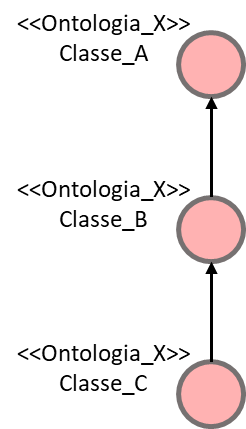
\includegraphics[scale=0.5]{3-notacao-visual-sawsdl/imagens/grafo-owl.png}
    \centering
    \caption[Representação visual em formato de grafo para classes OWL]{\textbf{Representação visual em formato de grafo para classes OWL.}}
    \label{fig:grafo-owl}
\end{figure}

Por fim, caso haja classes hierarquicamente dispostas entre duas outras classes OWL que são utilizadas em anotações semânticas e, consequentemente, já representadas visualmente no grafo, estas classes intermediárias são também visualmente representadas. Por exemplo, na \figurename~\ref{fig:grafo-owl}, caso as classes utilizadas em anotações semânticas sejam apenas as classes \texttt{Classe\_A} e \texttt{Classe\_C}, a classe \texttt{Classe\_B} será automaticamente representada visualmente, visto que ela encontra-se disposta hierarquicamente entre as duas outras classes. A representação visual de classes intermediárias independe da quantidade das mesmas.

%sejam representadas no grafo, por estarem sendo utilizadas em anotações semânticas, e estas duas classes possuírem alguma relação hierárquica, mesmo que seja por meio de outras classes intermediando esta relação, estas classes intermediárias são também visualmente representadas no grafo.
